%%%%%%%%%%%%%%%%%%%%%%%%%%%%%%%%%%%%%%%%%
% Journal Article
% LaTeX Template
% Version 1.3 (9/9/13)
%
% This template has been downloaded from:
% http://www.LaTeXTemplates.com
%
% Original author:
% Frits Wenneker (http://www.howtotex.com)
%
% License:
% CC BY-NC-SA 3.0 (http://creativecommons.org/licenses/by-nc-sa/3.0/)
%
%%%%%%%%%%%%%%%%%%%%%%%%%%%%%%%%%%%%%%%%%

%----------------------------------------------------------------------------------------
%	PACKAGES AND OTHER DOCUMENT CONFIGURATIONS
%----------------------------------------------------------------------------------------

%\documentclass[twoside]{article}
\documentclass{article}

\usepackage{lipsum} % Package to generate dummy text throughout this template

\usepackage[sc]{mathpazo} % Use the Palatino font
\usepackage[T1]{fontenc} % Use 8-bit encoding that has 256 glyphs
\linespread{1.05} % Line spacing - Palatino needs more space between lines
\usepackage{microtype} % Slightly tweak font spacing for aesthetics

\usepackage[hmarginratio=1:1,top=32mm]{geometry} % Document margins
%\usepackage{multicol} % Used for the two-column layout of the document
\usepackage[hang, small,labelfont=bf,up,textfont=it,up]{caption} % Custom captions under/above floats in tables or figures
\usepackage{booktabs} % Horizontal rules in tables
\usepackage{float} % Required for tables and figures in the multi-column environment - they need to be placed in specific locations with the [H] (e.g. \begin{table}[H])
\usepackage[hidelinks]{hyperref} % For hyperlinks in the PDF
\usepackage{amsmath}
\usepackage{graphicx}

\usepackage{lettrine} % The lettrine is the first enlarged letter at the beginning of the text
\usepackage{paralist} % Used for the compactitem environment which makes bullet points with less space between them

\usepackage{abstract} % Allows abstract customization
\renewcommand{\abstractnamefont}{\normalfont\bfseries} % Set the "Abstract" text to bold
\renewcommand{\abstracttextfont}{\normalfont\small\itshape} % Set the abstract itself to small italic text

\usepackage{titlesec} % Allows customization of titles
%\renewcommand\thesection{\Roman{section}} % Roman numerals for the sections
%\renewcommand\thesubsection{\Roman{subsection}} % Roman numerals for subsections
\titleformat{\section}[block]{\large\scshape\centering}{\thesection.}{1em}{} % Change the look of the section titles
\titleformat{\subsection}[block]{\large}{\thesubsection.}{1em}{} % Change the look of the section titles

\usepackage{fancyhdr} % Headers and footers
\pagestyle{fancy} % All pages have headers and footers
\fancyhead{} % Blank out the default header
\fancyfoot{} % Blank out the default footer
%\fancyhead[C]{Running title $\bullet$ November 2012 $\bullet$ Vol. XXI, No. 1} % Custom header text
\fancyfoot[RO,LE]{\thepage} % Custom footer text

%----------------------------------------------------------------------------------------
%	TITLE SECTION
%----------------------------------------------------------------------------------------

\title{\vspace{-15mm}\fontsize{24pt}{10pt}\selectfont\textbf{Statistické simulace pro měření operačních rizik}} % Article title


\usepackage[czech]{babel}

\author{
\large
\textsc{Edvard Špaček} \\
\normalsize Prognostický klub ČMA \\ % Your institution
\normalsize \href{mailto:edvard.spacek@gmail.com}{edvard.spacek@gmail.com} % Your email addres
\and
\large
\textsc{Jiří Špaček} \\
\normalsize ČVUT \\ % Your institution
\normalsize \href{mailto:jiri.spacek@fit.cvut.cz}{jiri.spacek@fit.cvut.cz} % Your email address
\and
\vspace{-5mm}
}
\date{}

%----------------------------------------------------------------------------------------

\begin{document}

\maketitle % Insert title

\thispagestyle{fancy} % All pages have headers and footers

%----------------------------------------------------------------------------------------
%	ABSTRACT
%----------------------------------------------------------------------------------------

%\begin{abstract}

%\noindent \lipsum[1] % Dummy abstract text

%\end{abstract}

%----------------------------------------------------------------------------------------
%	ARTICLE CONTENTS
%----------------------------------------------------------------------------------------

%\begin{multicols}{2} % Two-column layout throughout the main article text

\section{Cíl řešení}

\lettrine[nindent=0em,lines=3]{S} tatistické simulační řešení při nalezení složeného rozdělení ztrát (velikostí a četností), v \textbf{operačním riziku} bank/podniků, při aplikaci metod LDA (Loss Distrib. Approaches), implementace MC simulací, včetně \textbf{programového řešení} (vlastní model \textbf{MILDA\_E})



%------------------------------------------------

\section{SW závislosti}

\begin{compactitem}
\item Windows 7, Excel 2003 a nižší (vyšší verze nejsou odzkoušeny), Jensenovy simulační knihovny (k nalezení na webu)
\item knihovny ran\_var, simulation, simtools, instalované jako excelovské doplňky
\item funkce POISINV, LNORMINV Excelu (zkontrol.)
\item naše aplikace MILDA\_E
Pozn.: Pokud ohlásí modul Visual Basicu (Excel) chybu, většinou proto že není kompatibilita Jensenových knihoven s některou z dalších komponent systému. Jelikož knihovny nejsou dostupné, nelze udělat nápravu než vyměnit verze systému (s výhodou ve virtuálním stroji, což neruší stávající konfiguraci) a Excelu.
\end{compactitem}

V rámci řešení bylo popsáno zjednodušené řešení metodou Internal Measurement Approach (IMA), za předpokladu normálního rozdělení závažnosti (severity) ztrát  a Poissonova rozdělení četnosti ztrát. Číselné výsledky IMA metody lze použít pro porovnání s výstupy MC simulací.


\textbf{Hlavním problémem} implementace MC simulací je nalezení složeného rozdělení celkových ztrát podle metody LDA. Je třeba provést statistickou simulaci rozdělení hodnot celkových ztrát na základě simulací rozdělení četností (Poisson, variantně Binomial) a rozdělení hodnot jednotlivých ztrát (lognormal). Alternativou jsou náročnější analytické postupy výpočtu složeného rozdělení celkových ztrát (viz Panjer et al, 2004).
Hlavním výstupem v této části je realizace algoritmu metody MC v implementaci na \textbf{PC - modelu MILDA\_E}.


%------------------------------------------------

\section{Řešení problému LDA (se srovnávacími výpočty pomocí IMA) a popis předkládaného výpočetního programu MILDA\_E}

\subsection{Přehled zkoumaných AMA metod v rámci úkolu}

\begin{compactitem}
\item IMA (Internal Measurement Approach)				(1)
\item LDA (Loss Distribution Approach)				(2)
\end{compactitem}

Metody typu (1), (2) jsou statistického charakteru. Tento přístup sleduje výskyt ztrátových jevů a jejich velikost a měří je statistickými charakteristikami. Z těchto hodnot je v důsledku odvozována výše kapitálového příspěvku.


\subsection{Obchodní linie a typy rizik z hlediska statistického přístupu, agregace dílčích kapitálových požadavků}

Pro dosažení homogenity zpracování je celá oblast působnosti OR v bance rozdělena do matice. Týká se to i statistického popisu uplatňovaného metodami (1), (2).

\subsection{Stručná charakteristika používaných statistických AMA metod}


Pro tyto metody se vyžadují \emph{empiricky} naměřená ztrátová data. Jsou dále využívána pro účely \emph{validace} určitých teoretických rozdělení pravděpodobností a stanovení jejich parametrů. Validace se provádí formou otestování statistických \emph{hypotéz} o tom, že sledovaná data potvrzují platnost stanoveného typu rozdělení na dané hladině významnosti. Pro určení tvarů a parametrů rozdělení je třeba delší interval sledování  tak, aby výsledné odhady parametrů rozdělení ztrátových jevů vycházely z dostatečně četných pozorování.

Pro zpracování jsou brány v úvahu dva statistické znaky – \emph{výskyt} ztrátových jevů a jejich \emph{významnost} (hodnota). Tato rozdělení jsou odlišná pro oba aspekty ztrátových dat a liší se velikostí parametrů i mezi jednotlivými prvky matice tzv. obchodních linií a rizikových typů (ozn. maticí B/L $\times$ E/T). Bližší popis v metodice Basel II (na webu), je to na samostatné téma, zde pouze odkaz. Výpočet se ovšem vztahuje právě k této křížové struktuře. Pro úplnost je zmíněna i metoda IMA (Internal measurement approach). Metoda má přibližný charakter.

\textbf{(1) IMA} vychází z následujících vstupů:

\begin{compactitem}
    \item Celkový počet potenciálních ztrátových jevů
    \item Pravděpodobnost ztrátového jevu vrámci této množiny (četnost výskytu)
    \item Střední hodnota a směrodatná odchylka ztráty (velikost ztráty)
\end{compactitem}


IMA je charakterizována položením neočekávané ztráty jako násobku očekávané ztráty. \emph{Kapitálový} požadavek je dán neočekávanou ztrátou. Ta je odvozena jako součin:

\begin{compactitem}
    \item koeficientu gamma $\gamma$,
    \item indikátoru \emph{expozice} vůči riziku (potenciální výskyt ztrát),
    \item \emph{pravděpodobnosti} ztrátového jevu (z hlediska četnosti) a
    \item \emph{průměrné ztráty}, (z hlediska závažnosti)
\end{compactitem}

při dané konfidenční mezi (např. stanovena pro banky ve výši 99,9 \%).

Ve vzorci se objevují dva typy rozdělení, pro četnost ztrátových jevů a velikost ztrát. Analyticky je využíváno binomické (pro menší četnost výskytu) resp. Poissonovo rozdělení.  Pro hodnotu ztrát je využíváno normální rozdělení.

\textbf{(2) Metody typu LDA} vycházejí z přímého měření neočekávané ztráty jako charakteristiky \emph{složeného rozdělení četností} a závažností ztrát. Jako typ rozdělení hodnot ztrát se využívá \emph{lognormální} rozdělení. Četnosti výskytu ztrátových jevů jsou opět binomické, resp. Poissonovy. Neočekávaná ztráta je kvantifikována jako 99,9 \% kvantil složeného rozdělení pravděpodobností minus očekávaná ztráta. Kapitálový požadavek je tedy vypočten z charakteristik složeného rozdělení.

Při uplatnění LDA postupu je základní problém \emph{výpočet složeného rozdělení}. Vrámci tohoto postupu je třeba jmenovité hodnoty velikostí skládat s četnostmi výskytu.


\subsection{Stručný algoritmus výpočtu podle IMA}

Vychází se z počtu $N$ událostí, potenciálně zatížených op-rizikem v ročním horizontu. Dále z \emph{pravděpodobnosti} ztrátového jevu $p$ ztěchto $N$ možných událostí.
Základem je odhad \emph{očekávaných} ztrát $N * p * \mu_L$. K tomu je potřeba odhadnout průměrnou ztrátu z jedné události $\mu_L$. Tato charakteristika je počítána ze dvou zdrojů, rozdělení:

\begin{itemize}
  \item A) Četnosti (frequency) ztrát (binomické rozdělení); parametry $N$, $p$
  \item B) Velikosti (severity) ztrát (normální rozd.); parametry $\mu_L$, $\sigma_L^2$ (stř. hodnota, rozptyl)
\end{itemize}

Propočty z rozdělení $A$ a $B$ a jejich charakteristik získáme velikosti $\gamma$ z hodnoty součinitele $k$. IMA je charakterizována pevnou velikostí rozdílu mezi \emph{očekávanou} (průměr rozdělení) a \emph{neočekávanou} ztrátou (chvost rozdělení daný 99,9 \% věrohodností).

V teorii se odvozují vzorce:

\begin{equation}
  \gamma = k * \frac{\sqrt{1 + (\frac{\sigma_L}{\mu_L})^2}}{\sqrt{N * p}}
\end{equation}

kde $k = \frac{(\alpha \textrm{ percentil rozd. } B - N * p)}{\sigma_L}$

Jednodušší tvar vzorce je (při neznámém rozptylu $\sigma_L$):

\begin{equation}
  \begin{aligned}
  \gamma &= \frac{k}{\sqrt{N * p}} \\
       k &= k * \mu_L \sqrt{N * p}
  \end{aligned}
\end{equation}

Alternativní rozdělení k $A$ (četnosti) je Poissonovo, k $B$ (ztráty) lognormální.

\textbf{Výpočet kapitálového požadavku}

Kapitálový požadavek k OR je dán neočekávanou ztrátou, očekávaná je kryta rezervami, které lze apriori vyčlenit. Ta je odvozena s pomocí koeficientu $\gamma$, indikátoru expozice $EI$ vůči riziku, pravděp. ztrátového jevu $PE$ a průměrné ztráty $LGE$, $I$, $J$ ozn. linii/typ, $K$ ozn. kapitálový požadavek.

\begin{equation}
  K_{i,j} = \gamma_{i,j} * EI_{i,j} * PE_{i,j} * LGE_{i,j} = \gamma_{i,j} * EL_{i,j}
\end{equation}


Výpočet podle IMA algoritmu je brán orientačně, jako vodítko pro účely porovnání výsledků s metodou LDA, jejíž výsledky jsou brány jako směrodatné.



\subsection{Stručný algoritmus výpočtu podle LDA}

Cílem je vytvořit model pro agregované ztráty - stanovit rozdělení pravděpod. pro celkovou ztrátu.

\emph{Celková ztráta} $S$ je definovaná jako suma:

\begin{equation}
  S = X_1+…+X_N (N = 0,1,2 \ldots)
\end{equation}
  
náhodného počtu $N$ jednotlivých ztrát ($X_1 \ldots X_N$). Je zaveden předpoklad nezávislosti a stejného rozdělení $X_i$. Rovněž $N$ a $X_i$ jsou nezávislé. Tzn.:

\begin{compactitem}
\item Za předpokladu $N = n$ náh. veličiny $X_1 \ldots X_n$ jsou nezávislé a stejně rozdělené
\item Rozdělení $N$ nezávisí na hodnotách $X_1,X_2 \ldots$.
\end{compactitem}
  
Problematika výpočtu se soustřeďuje na:
\begin{compactitem}
\item Odhad rozdělení pravděpodobností pro $N$ založený na náh. výběru
\item Odhad rozdělení pravděpodobností pro $X_j$ založený na náh. výběru
\item S využití těchto rozdělení zkonstruovat rozdělení náh. veličiny $S$
\item Rozdělení (4.3) nazývá se složeným rozdělením.
\end{compactitem}


\begin{figure}[H]
  \caption{LDA charakteristiky, viz čl. EVT-box}
  \centering
    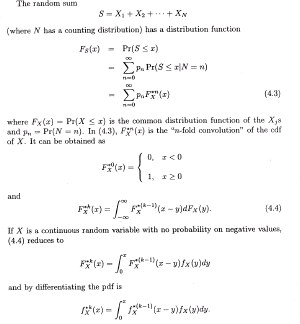
\includegraphics[width=0.6\textwidth]{ldachar}
\end{figure}


%% The random sum

%% \begin{equation}
%%   S = X_1 + X_2 + \cdots + X_N
%% \end{equation}

%% (where $N$ has a counting distribution) has a distribution function

%% \begin{equation}
%%   \begin{aligned}
%% F_s(x) &= P_x(S \leq x) \\
%%       &= \sum_{n=0}^{\infty}p_nP_x(S \leq x | N = n) \\
%%       &= \sum_{n=0}^{\infty}p_nF_X^n\{x\}
%%       \end{aligned}
%% \end{equation}

%% where $F_X(x) = P_x\{X \teq x\}$ is the common distribution function of the $X_j$ and $p_n = Px\{N = n\}$. In (d.3), $F_x^n\{x\}$ is the n-fold convolution of the cdf of $X$. It can be obtained as

%% smth

%% and

%% F_X^{\lambda}(X) = \int_{-\infty}^{\infty}

\subsection{Simulační metoda}
Cílem je stanovit \emph{empirickou} funkci rozdělení na základě posloupnosti (pseudo) náhodných čísel $s_1, \ldots s_n$. Je jasné, že se vzrůstem počtu hodnot lze logicky docílit přesnějšího odhadu. Rizikový horizont je zpravidla brán u operačních rizik jako roční. V programu je provedeno \emph{1000 simulací}. Jako hledané charakteristiky rozdělení bereme empirické hodnoty jejich odhadů (např. výběrové průměry, směrodat. odchylky, kvantily apod.). Intervaly spolehlivosti odhadů nejsou zahrnuty do výpočtu.


%------------------------------------------------

\section{Implementace MC simulací}


\subsection{Excelovský program „MILDA\_E – Malý Ima LDA kalkulátor (Excel)“}

Seznam a funkčnost pracovních sheetů:
\begin{compactitem}
\item \textbf{Výběr}: nabídne seznam BL/ET (matice k8x7 u bank), po
  provedení výběru uživatelem se přesune do sheetu:
\item \textbf{Vstupy\_a\_Výstupy}: pro zvolenou kombinaci BL/ET se zavádí vstupy a výpočet výstupních hodnot
\emph{vstupy} – počet ztrátových jevů $N$, pravděpodobnost ztrát. jevu $p$, koeficient $\lambda$ Poissonova rozdělení, průměrná ztráta a rozptyl rozdělení ztrát, konfidenční mez $\alpha$,
\emph{výstupy} IMA – kapitálový příspěvek typu \textbf{a} (se znalostí rozptylu závažnosti ztráty) a \textbf{b} (bez znalosti rozptylu závažnosti ztráty), očekávaná celková ztráta
  
Sheet obsahuje programové tlačítko LDA, které posouvá výpočet do další \textbf{simulační fáze}.
\item \textbf{Poisson\_distr.}: obsahuje výpočty na základě Poissonova rozdělení
Oba poslední sheety jsou doplněny Normálním rozdělením závažností ztrát.
\item \textbf{Simulace}: Je sheetem ve kterém se provádějí výpočty složeného rozdělení. Jsou vygenerovány (pomocí pseudonáhodných čísel) a zobrazeny empirické rozdělení četností a velikostí ztrát. Problematika výpočtu se soustřeďuje na generování náhodných horních mezí pro součtové hodnoty sn. Byl připraven algoritmus, který náhodná čísla vygenerovaná z Poissonova rozdělení výskytů převádí na výpočet náhodných horních mezí pro součtové buňky. Tyto součtové hodnoty (v souhrnném vyjádření) vytvářejí empirické rozdělení agregovaných ztrát. Dále jsou propočteny střední hodnota, směrodatná odchylka, 0,999 percentil a  odvozeně opr. položky, kapitálový příspěvek pro krytí operačních rizik.
\item \textbf{Simulace (2)}: je sheetem ve kterém se provádí zobrazení vypočtených hodnot charakteristik složeného rozdělení
\end{compactitem}

\subsection{Programové charakteristiky}

Výpočet využívá statistických a vyhledávacích funkcí Excelu, včetně maker Visual Basicu v rámci Excelu. Výpočet je podpořen řadou simulačních knihoven pro vygenerování pseudonáh. čísel z předepsaných rozdělení. Není omezením (vzhledem k využití dalších analytických funkcí) výpočet Binomického rozdělení pro velkou hodnotu součinu $N * p$, rovněž Poissonova $r$. pro vysoké $\lambda$. Je však omezením takové hodnoty použít pro výpočet simulací. Pro $\mu$, $\sigma$ není omezení hodnot algoritmem vyžadováno.



\subsection{Vstupní/výstupní sheety aplikace MILDA\_E}

\begin{figure}[H]
  \caption{Matice BL $\times$ ET}
  \centering
    
\includegraphics[width=0.75\textwidth]{matice}
\end{figure}


\begin{figure}[H]
  \caption{Součtová tabulka rizik. kapitálu}
  \centering
    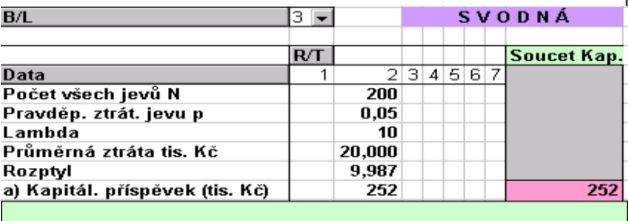
\includegraphics[width=0.75\textwidth]{tabulka}
\end{figure}

\begin{figure}[H]
    \caption{Vstupní param. Poissonova (aktivní, červené zadání) a lognormálního rozd., vstup do výpočtu „LDA“}    
  \centering
    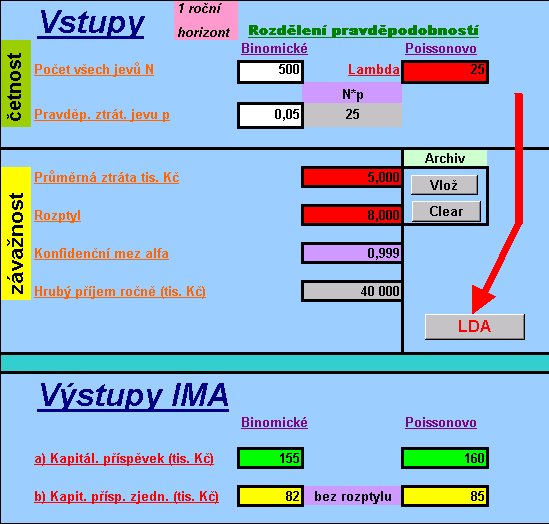
\includegraphics[width=0.75\textwidth]{vstup}

\end{figure}

\begin{figure}[H]
  \caption{Ovládací tlačítko výpočtu „simuluj“, simulační graf a rizikové charakteristiky (rizikový kapitál)}
  \centering
    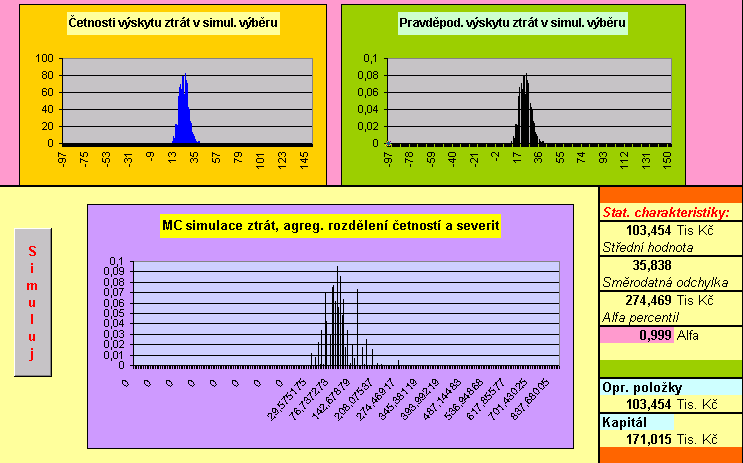
\includegraphics[width=0.75\textwidth]{simuluj}
\end{figure}


%----------------------------------------------------------------------------------------

%\end{multicols}

\end{document}
